\documentclass[conference]{IEEEtran}
\IEEEoverridecommandlockouts

\usepackage{cite}
\usepackage{amsmath}
\usepackage{graphicx}
\usepackage{booktabs}
\usepackage{xcolor}
\usepackage[hyphens]{url}

\graphicspath{{../results/}}

% Open items. \todo{...} marks a missing source or check; TODO-RESULT marks a missing number.
\newcommand{\todo}[1]{\textcolor{red}{[TODO: #1]}}

% numbers.tex -- every numeric result used in main.tex, defined once (draft 3).
% Source of every value: papers/benchmark/results/summary.md, regenerated by
% experiments/summarize.py from results/raw/*.csv (pass 3, real protocol
% implementations). Each macro names the summary.md section ("S:") and the CSV
% behind it ("CSV:"). Values from papers/benchmark/budget-evidence.md say so.
% Missing values print as TODO-RESULT (red). No number is typed in main.tex.

\newcommand{\missing}{\textcolor{red}{TODO-RESULT}}

% ---------------------------------------------------------------- run tags
% S: header "Code commit" + run-tag table; CSV: every raw/*.csv (machine/date/git_commit/git_dirty columns)
\newcommand{\RunMachine}{cloud-vm-4core}
\newcommand{\RunDate}{2026-11-13}
\newcommand{\RunCommit}{694ba76}   % short form of 694ba76f1ed7be05e6b07c01ca0cba0d8749a78e (git_dirty = 0)
\newcommand{\RunCommitFull}{694ba76f1ed7be05e6b07c01ca0cba0d8749a78e}
\newcommand{\RunCores}{4}          % S: run-tag table, machine name "cloud-vm-4core"
\newcommand{\RunCPU}{\missing}     % CPU model / OS of the VM: not in summary.md
\newcommand{\LibOQSVersion}{0.16.0}% S: Part A; CSV: raw/sizes_declared.csv
\newcommand{\OpenSSLVersion}{3.0.13}% S: Part A classical table; CSV: raw/classical_timing_cloud-vm-4core.csv
\newcommand{\IterFast}{10\,000}    % S: Part A timing table (iterations); CSV: raw/oqs_timing_cloud-vm-4core.csv
\newcommand{\IterSlow}{100}        % same; SLH-DSA, CROSS, MQOM rows
\newcommand{\NumTimed}{57}         % S: Part A, schemes timed; CSV: raw/oqs_timing_cloud-vm-4core.csv

% ---------------------------------------------------------------- scheme set
% S: Part A "liboqs 0.16.0: ..."; CSV: raw/sizes_declared.csv
\newcommand{\NumParamSets}{221}    % signature parameter sets enabled
\newcommand{\NumClasses}{64}       % distinct (family, level, pk size, sig size) classes
\newcommand{\NumClassesLow}{24}    % lowest-level classes (main tables)
\newcommand{\NumStateful}{5}       % S: Q1 "LMS/XMSS: 5 literature size-only rows"; CSV: results/main_table_lowest_level.csv
\newcommand{\LMSSigsPerKey}{32}    % S: Q1 LMS/XMSS paragraph (H = 5)
\newcommand{\LMSBSMTime}{3.2\,s}   % S: Q1 LMS/XMSS paragraph (32 signatures of 10 Hz BSMs)
\newcommand{\LMSHigh}{\missing}    % S: Q1 LMS/XMSS paragraph, H = 15/20 rows are TODO-RESULT

% ---------------------------------------------------------------- Part A sizes and timings
% S: Part A timing table; CSV: raw/sizes_declared.csv, raw/oqs_timing_cloud-vm-4core.csv
\newcommand{\SigFalcon}{752}       % Falcon-512 sig_declared
\newcommand{\PkFalcon}{897}        % Falcon-512 length_public_key
\newcommand{\SigFalconPad}{666}    % Falcon-padded-512 sig_declared
\newcommand{\SigMLDSA}{2420}       % ML-DSA-44 sig_declared
\newcommand{\SigMAYOone}{454}      % MAYO-1
\newcommand{\SigSNOVA}{248}        % SNOVA_24_5_4
\newcommand{\SigOVIs}{96}          % OV-Is
\newcommand{\SigSLHs}{7856}        % SLH_DSA_PURE_SHA2_128S
\newcommand{\SignMedFalcon}{235}   % Falcon-512 sign median 234.7 us (rounded)
\newcommand{\SignMedMLDSA}{68}     % ML-DSA-44 sign median 67.68 us (rounded)
\newcommand{\SignMedSLHs}{591}     % SLH_DSA_PURE_SHA2_128S sign median 5.913e+05 us, in ms

% ---------------------------------------------------------------- profiles
% S: "Assumed and sourced parameters" profile table; CSV: experiments/profiles.yaml
% (as printed in summary.md); derivations in budget-evidence.md
\newcommand{\CeilRID}{255}  \newcommand{\BudRID}{201}   % RFC 9575 cap (budget-evidence.md remote_id)
\newcommand{\CeilSIB}{372}  \newcommand{\BudSIB}{293}   % 372 - 79 B SIB1 (budget-evidence.md sib1)
\newcommand{\SIBUsed}{79}                               % budget-evidence.md sib1; S: slot table "app bytes 79 B"
\newcommand{\CeilOS}{208}                               % 16 x 104 bit
\newcommand{\BudKROOT}{158}                             % derived, DSM-KROOT signature space
\newcommand{\BudPKR}{76}                                % derived, (1632-1024) bit / 8, DSM-PKR key space
\newcommand{\CeilCV}{437}   \newcommand{\BudCV}{374}    % derived: 437 - 24 SPDU hdr - 39 BSM core
\newcommand{\CeilJ}{2481}   \newcommand{\BudJ}{2414}    % derived: 2481 - 28 hdr - 39 BSM core
\newcommand{\CeilDNS}{1232} \newcommand{\BudDNS}{1232}  % whole-message recommendation
\newcommand{\HdrSPDUCV}{24}                             % S: "C-V2X budget rule" (twardokus2024when)
\newcommand{\HdrJ}{28}                                  % S: "C-V2X budget rule" (abrar2026deployment)
\newcommand{\BSMCore}{39}                               % S: "C-V2X budget rule" (abrar2026deployment)
\newcommand{\FrameCV}{40}                               % S: "C-V2X budget rule" (frame overhead, subtracted from neither)
\newcommand{\BudCVSens}{334}                            % S: "C-V2X 437 sensitivity" row
\newcommand{\FitCVSens}{8}                              % S: Q1 "Sensitivity of cv2x_437": 8/24 at 374 B and at 334 B
\newcommand{\BSMSizeCV}{\missing}                       % S: "Runs still needed": BSM size for 437 B
\newcommand{\PerRID}{3\,s}  \newcommand{\PerSIB}{0.16\,s}
\newcommand{\PerOS}{480\,s} \newcommand{\PerCV}{0.1\,s}
\newcommand{\PerDNS}{\missing}                          % dns message period TODO-RESULT in summary.md
\newcommand{\DeadRID}{30\,s} \newcommand{\DeadSIB}{10\,s} % assumed join deadlines (profile table)
\newcommand{\DeadOS}{720\,s} \newcommand{\DeadCV}{10\,s}
\newcommand{\DeadDNS}{1\,s}
\newcommand{\HdrSrc}{\missing}                          % S: "Runs still needed": per-message fragment-header sizes of the sources
\newcommand{\CertMeta}{\missing}                        % S: parameter table "certificate metadata"
\newcommand{\CertMetaLo}{41}  \newcommand{\CertMetaHi}{73}  % S: same row, sensitivity values (derived)
\newcommand{\CertClFixed}{105}                          % S: "classical-issuer certificate P + 105 B"
\newcommand{\CertDigest}{8}                             % S: slot table, digest bytes (cv2x)
\newcommand{\CertEvery}{5}                              % S: slot table, certificate every 5th slot

\newcommand{\TabProfileRows}{%
Remote ID          & \CeilRID & \BudRID        & \PerRID & \DeadRID & \cite{wiethuechter2024drip} \\
5G SIB1            & \CeilSIB & \BudSIB        & \PerSIB & \DeadSIB & \cite{darzi2026a} \\
OSNMA KROOT (sig.) & \CeilOS  & \BudKROOT$^*$  & \PerOS  & \DeadOS  & \cite{junquera2023assessment} \\
OSNMA PKR (key)    & \CeilOS  & \BudPKR$^*$    & \PerOS  & --       & \cite{junquera2023assessment} \\
C-V2X 437$^\dagger$   & \CeilCV  & \BudCV$^*$  & \PerCV  & \DeadCV  & \cite{twardokus2024when} \\
C-V2X J3161$^\dagger$ & \CeilJ   & \BudJ$^*$   & \PerCV  & \DeadCV  & \cite{abrar2026deployment} \\
DNS$^\dagger$         & \CeilDNS & \BudDNS     & \PerDNS & \DeadDNS & \cite{goertzen2022post} \\
}

% ---------------------------------------------------------------- Q1
% S: Q1 "Totals over the lowest-level liboqs classes", "PQ-issuer certificate fits",
% "classical-issuer case", chain join-time table; CSV: raw/scoring_all_levels.csv,
% results/main_table_lowest_level.csv. Columns: RID, SIB1, KROOT, CV437, J3161, DNS (of 24).
\newcommand{\TabQOneRows}{%
full                         & 7  & 8  & 5 & 8 & 11      & 11 \\
hybrid                       & 5  & 7  & 0 & 8 & 11      & 11 \\
cert., PQ issuer$^a$         & -- & -- & --& 0 & 4/3/3   & -- \\
cert., classical issuer      & -- & -- & --& 0 & 4       & -- \\
signature + bare key         & 0  & -- & --& --& --      & 0 \\
chain join $\le$ deadline    & 11 & 23 & 0 & 24& 24      & n/a \\
}
\newcommand{\FullFitMin}{5}        % osnma_kroot158
\newcommand{\FullFitMax}{11}       % cv2x_j3161, dns
\newcommand{\KeyFitPKR}{9}         % S: Q1 "OSNMA key delivery": 9/24
\newcommand{\CertPQJ}{4}           % full_cert_pq J3161 at metadata 0
\newcommand{\CertPQJmeta}{3}       % at metadata 41 and 73
\newcommand{\CertClJ}{4}           % full_cert_cl J3161
% chain join (static, no loss): S: Q1 chain join-time table
\newcommand{\JoinOSmin}{810\,s}    \newcommand{\JoinOSmax}{$5.652\times10^{4}$\,s}  % 5.652e+04 s
\newcommand{\JoinRIDmet}{11}       \newcommand{\JoinRIDmax}{276\,s}
% Margins on J3161 (S: Q1 margins table; CSV: results/main_table_lowest_level.csv)
\newcommand{\MarFalconJ}{1662}     % full, Falcon-512, cv2x_j3161 (full-signature table)
\newcommand{\MarFalconJpq}{13}     % full_cert_pq, Falcon-512
\newcommand{\MarFalconJcl}{660}    % full_cert_cl, Falcon-512
\newcommand{\MarMLDSAJ}{$-6$}        % full, ML-DSA-44, cv2x_j3161
\newcommand{\MsgFalconCV}{3}       % full, Falcon-512, cv2x_437: 3 msg
\newcommand{\MarFalconCV}{$-378$}    % margin, Falcon-512, cv2x_437
\newcommand{\MsgMLDSAsib}{9}       \newcommand{\TimeMLDSAsib}{1.28\,s}   % full, ML-DSA-44, sib1
\newcommand{\MsgMLDSArid}{13}      \newcommand{\TimeMLDSArid}{36\,s}     % full, ML-DSA-44, remote_id
\newcommand{\MsgFalconKR}{5}       \newcommand{\TimeFalconKR}{$2.28\times10^{3}$\,s} % full, Falcon-512, osnma_kroot158
% consistency checks (S: Q1 "Consistency checks of stated numbers")
\newcommand{\DarziFnPkts}{13}      \newcommand{\DarziMlPkts}{34}
\newcommand{\JunqComputed}{68}     \newcommand{\JunqReported}{67}
% reproductions not done (S: "Runs still needed", items not implemented)
\newcommand{\DarziOTARepro}{\missing}    % darzi2026a 324/744 B OTA overhead
\newcommand{\DarziTenRepro}{\missing}    % darzi2026a 10%-loss success point
\newcommand{\JunqueraKeyRepro}{\missing} % junquera2023assessment 71-block key figure
\newcommand{\GoertzenRepro}{\missing}    % goertzen2022post transfer bytes
\newcommand{\YoshizawaRepro}{\missing}   % yoshizawa2026a ZK compression
\newcommand{\ChenRepro}{\missing}        % chen2025hybrid size tables

% ---------------------------------------------------------------- Q2 setup
% S: Q2 header, parameter table and allocation tables; CSV: raw/proto_results_cloud-vm-4core.csv,
% raw/proto_alloc_cloud-vm-4core.csv
\newcommand{\NumModes}{10}         % frag_rep, frag_mds, hyb_rep, hyb_mds, merkle4/8/16, chain, chain_lead, chain_lead_cont
\newcommand{\NumProtoPQ}{7}        % PQ schemes in the protocol runs
\newcommand{\NumProtoRows}{100\,800}
\newcommand{\Seeds}{20}
\newcommand{\NMsgs}{80}            % messages per run
\newcommand{\EpochE}{20}           % windows per epoch
\newcommand{\Mmain}{10}  \newcommand{\Mbig}{40}
\newcommand{\TagB}{16}             % tag, disclosed key, commitment (16 B each), timestamp 4 B
\newcommand{\TsB}{4}
\newcommand{\PathHashB}{32}        % Merkle path hash
\newcommand{\RSmax}{255}           % zfec n <= 255
\newcommand{\ZfecVersion}{1.6.0.0}
\newcommand{\SlotSIB}{293}  \newcommand{\SlotCV}{366}  \newcommand{\SlotJ}{2406}   % slot capacity (regular)
\newcommand{\WinSIB}{1600}  \newcommand{\WinCV}{1000}                            % window ms at M = 10 (S: SLH-DSA table)
\newcommand{\AllocSIB}{2930}                                                       % B allocated per message, sib1
\newcommand{\HdrProtoLo}{3} \newcommand{\HdrProtoHi}{11}   % S: "Runs still needed": explicit headers 3-11 B
\newcommand{\ProtoMaxFrameSIB}{293}

% ---------------------------------------------------------------- Q2 verdicts
% S: Q2 "Hypothesis tests"; CSV: results/q2_verdicts.csv
\newcommand{\CellsShare}{462}  \newcommand{\CellsOther}{440}
\newcommand{\HaW}{118} \newcommand{\HaL}{3}   \newcommand{\HaT}{341}
\newcommand{\HbW}{131} \newcommand{\HbL}{290} \newcommand{\HbT}{19}
\newcommand{\HcW}{0}   \newcommand{\HcL}{440} \newcommand{\HcT}{0}
\newcommand{\HdW}{25}  \newcommand{\HdL}{385} \newcommand{\HdT}{30}
\newcommand{\HaInfeas}{22}         % S: "H2a detail": wins where frag_mds is infeasible
\newcommand{\HaRuns}{96}           % wins where frag_mds runs
\newcommand{\HaLossScheme}{Falcon-512} % S: "Chain loses share in 3 cells; Falcon-512 3"
\newcommand{\HaWsib}{51} \newcommand{\HaWcv}{51} \newcommand{\HaWj}{16}  % S: per-profile table, share wins
\newcommand{\HaLj}{3}
\newcommand{\TabVerdictRows}{%
H2a share $\uparrow$      & \CellsShare & 118/3/341  & 118/3/341 & 118/3/341 & supported \\
H2b B/auth.\ msg $\downarrow$ & \CellsOther & 131/290/19 & 124/309/7 & 100/324/16 & refuted \\
H2c delay $\downarrow$    & \CellsOther & 0/440/0    & 0/440/0   & 0/440/0   & refuted \\
H2d join $\downarrow$     & \CellsOther & 25/385/30  & 0/439/1   & 0/439/1   & refuted \\
}
% S: "Reading H2b"
\newcommand{\ByteRatioMed}{1.132} \newcommand{\ByteRatioLo}{0.706} \newcommand{\ByteRatioHi}{1.599}
\newcommand{\BytePairs}{19}
% S: target-share table (share >= 0.95 at M = 10, of 21 (profile, PQ) pairs)
\newcommand{\TgtPairs}{21}
\newcommand{\TgtFragMDS}{17} \newcommand{\TgtFragMDSbig}{4}
\newcommand{\TgtChain}{21}   \newcommand{\TgtMerkleFour}{19}

% ---------------------------------------------------------------- Q2 cells quoted in text
% S: Q2 share tables (proto_summary.csv)
\newcommand{\ShMLsibFragTen}{0.721}   % sib1 iid 0.1, ML-DSA-44 frag_mds
\newcommand{\ShMLcvFragThirty}{0.247} % cv2x_437 iid 0.3, ML-DSA-44 frag_mds
\newcommand{\ShMLsibFragThirty}{0.142}% sib1 iid 0.3, ML-DSA-44 frag_mds
\newcommand{\ShMLsibFragGE}{0.539}    % sib1 GE 0.3/b10, ML-DSA-44 frag_mds
\newcommand{\ShFalsibFragGE}{0.830}   % sib1 GE 0.3/b10, Falcon-512 frag_mds
\newcommand{\ShChainsibGE}{0.888}     % sib1 GE 0.3/b10, chain
\newcommand{\ShMerkleEightsibGE}{0.790}% sib1 GE 0.3/b10, merkle8
\newcommand{\ShOVsibFragGE}{0.892}    % sib1 GE 0.3/b10, OV-Is frag_mds
% S: Q2 "Delay, join time, bytes and CPU at iid loss 0.1 (M = 10)", sib1 block
\newcommand{\TabQTwoRows}{%
ML-DSA-44  & frag\_mds  & 0.721 & 1512  & 2872  & 3807 \\
           & merkle4    & 1.000 & 6624  & 6576  & 2910 \\
           & merkle16   & 1.000 & 25760 & 25480 & 2860 \\
           & chain      & 1.000 & 1760  & 1856  & 2885 \\
           & chain\_lead\_cont & 1.000 & 1760 & 17376 & 2965 \\
\midrule
Falcon-512 & frag\_mds  & 1.000 & 480   & 584   & 2550 \\
           & merkle4    & 1.000 & 6560  & 6080  & 2590 \\
           & chain      & 1.000 & 1760  & 1080  & 2375 \\
           & chain\_lead\_cont & 1.000 & 1760 & 17376 & 2685 \\
\midrule
OV-Is      & frag\_mds  & 1.000 & 160   & 176   & 1010 \\
           & merkle4    & 1.000 & 6560  & 5840  & 1680 \\
           & chain      & 1.000 & 1760  & 1032  & 1615 \\
}
% S: Merkle trade-off table, sib1 Falcon-512 (proto_summary.csv)
\newcommand{\MerkFourDelay}{6560} \newcommand{\MerkSixteenDelay}{25760}
% S: "Burst loss" table (GE minus iid share, mean over profiles and PQ schemes), p0.3/burst10
\newcommand{\BurstChain}{$-0.119$} \newcommand{\BurstFragMDS}{$-0.076$}
\newcommand{\BurstMerkleEight}{$-0.223$} \newcommand{\BurstFragRep}{$-0.041$}
% S: "Closed forms as a cross-check"; CSV: raw/loss_crosscheck_cloud-vm-4core.csv
\newcommand{\XCells}{1716} \newcommand{\XOut}{0} \newcommand{\XMaxDiff}{0.0175}
% S: "Negative tests"; CSV: raw/negative_tests_cloud-vm-4core.csv
\newcommand{\NegPassed}{427} \newcommand{\NegRuns}{427}
\newcommand{\NegCtrl}{21}          % T4-control: forgeries accepted without the time-safety check (21/21)
\newcommand{\NegE}{8} \newcommand{\NegN}{32}
% S: "Real-UDP mode"; CSV: raw/udp_smoke_cloud-vm-4core.csv
\newcommand{\UDPSame}{4} \newcommand{\UDPRuns}{4}
% S: "SLH-DSA-128s (reported, not dropped)"
\newcommand{\SLHInfeas}{8} \newcommand{\SLHConfigs}{24}
\newcommand{\SLHSlowSender}{0}   % configurations with tx_realtime_ratio > 1
\newcommand{\SLHSignOverSlot}{24}% configurations whose sign time exceeds one slot
\newcommand{\RTCheckSlow}{0} \newcommand{\RTCheckN}{202}  % S: Q3 "Sender real-time check"

% ---------------------------------------------------------------- Q2 loss grid and decision rule
% S: parameter table "loss" row and "Hypothesis tests" rule paragraph
\newcommand{\LossGrid}{0.02, 0.05, 0.1, 0.2, 0.3}   % i.i.d. slot loss
\newcommand{\LossMaxPct}{30\%}
\newcommand{\GEStat}{0.1, 0.2, 0.3}                 % GE stationary loss (burst table)
\newcommand{\GEBursts}{3, 5, 10}                    % mean burst lengths, slots
\newcommand{\GEBurstMax}{10}  \newcommand{\GELossMax}{0.3}
\newcommand{\LossTen}{0.1}    \newcommand{\LossThirty}{0.3}
\newcommand{\RuleSE}{3}                             % |mean d| > 3 SE
\newcommand{\RuleMinShare}{0.005}                   % minimum effect, share
\newcommand{\RuleMinRel}{1\%}                       % minimum effect, bytes / delay / join
\newcommand{\RuleFactor}{2}                         % supported if wins >= 2 x losses
\newcommand{\TgtShare}{0.95}                        % S: target-share table
\newcommand{\MerkleN}{4, 8, 16}

% ---------------------------------------------------------------- source facts (budget-evidence.md)
\newcommand{\TwMHz}{10}            % twardokus2024when: 437 B in a 10 MHz channel
\newcommand{\AbMHz}{20}            % abrar2026deployment: J3161 20 MHz profile
\newcommand{\AbMCS}{11}            % MCS 11
\newcommand{\AbSubch}{10}          % 10 subchannels
\newcommand{\AbPDR}{90\%}          % PDR target met only at LOS level of service A
\newcommand{\RIDDynPer}{1\,s}      % RFC 9575 dynamic (DRIP Wrapper) period
\newcommand{\RIDFrame}{25}         % Bluetooth 4.x payload per frame (RFC 9575)
\newcommand{\OSBlockBits}{104}     % OSNMA DSM block, bits
\newcommand{\OSBlocks}{16}         % blocks per DSM
\newcommand{\OSKROOTbits}{79}      % bits per block, DSM-KROOT DS field (source figure)

% ---------------------------------------------------------------- Q3
% S: Q3 table and verdict; CSV: raw/oqs_timing_cloud-vm-4core.csv, raw/scoring_all_levels.csv
\newcommand{\QThreeSize}{7} \newcommand{\QThreeTime}{0} \newcommand{\QThreeND}{1}
\newcommand{\QThreeFams}{8}

% ---------------------------------------------------------------- misc values quoted in text
\newcommand{\ShChainOne}{1.000}   % S: Q2 share tables, chain at sib1 iid 0.1 and cv2x_437 iid 0.3 (ML-DSA-44 rows)
\newcommand{\MerkFourN}{4} \newcommand{\MerkSixteenN}{16}  % S: Merkle trade-off table (n)
\newcommand{\BSMHz}{10}           % S: Q1 LMS/XMSS paragraph ("10 Hz BSMs")
\newcommand{\DarziLossPct}{10\%}  % budget-evidence.md sib1 (d): darzi2026a success at 10% loss
\newcommand{\CertMetaUsed}{0}   % S: parameter table, certificate metadata (0 used = lower bound)
\newcommand{\InfeasShare}{0}    % S: hypothesis rule, infeasible mode has share 0


\begin{document}

\title{Which Post-Quantum Signature Modes Fit Broadcast Budgets?\\
A Cross-Domain Scoring of Authentication Modes\\ for Handshake-Free Cyber-Physical Broadcasts}

\author{\IEEEauthorblockN{Author Name}
\IEEEauthorblockA{Affiliation}}

\maketitle

\noindent\fbox{\parbox{\dimexpr\columnwidth-2\fboxsep-2\fboxrule}{%
\centering\textbf{\textcolor{red}{DRAFT -- PROVISIONAL SMOKE-TEST NUMBERS}}\\[2pt]
\footnotesize\raggedright
All measurements come from smoke runs on a shared cloud VM (machine tag
\texttt{\RunMachine}, \RunDate, commit \texttt{\RunCommit}) with
\IterFast{} iterations (\IterSlow{} for slow schemes). They are not
publication numbers. Every value is defined in \texttt{numbers.tex} and
traced to \texttt{results/summary.md}; open items are marked
\textcolor{red}{TODO-RESULT} or \textcolor{red}{[TODO]}.}}

\begin{abstract}
Broadcast channels in cyber-physical systems (vehicle-to-vehicle messages,
drone Remote ID, satellite navigation message authentication, cellular
system information, DNS responses) cannot run a handshake, and each has a
hard per-message byte budget. Prior post-quantum (PQ) studies fit
signatures to one such budget at a time. We score one set of
authentication modes (full signature, signature with certificate,
fragmented signature, a PQ-anchored symmetric key chain, and a
classical/PQ hybrid) against five budget profiles from five domains, using
signature sizes and timings measured with liboqs~\LibOQSVersion{} on x86.
In this provisional data, a full PQ signature fits in \QOneFullFit{} of
\QOnePairs{} (parameter set, profile) pairs, all of them UOV, SNOVA,
MAYO or Falcon; no parameter set fits when a same-scheme certificate is
attached. A loss model comparing the PQ-anchored chain to fragmented
signatures at 0--30\% i.i.d.\ loss favours the chain on bytes per
verified message and 95th-percentile time to authenticate, but not on
verified share at low loss, and depends on assumed chain parameters; we
report it as inconclusive. On x86, signature size, not the sign/verify
timing tail, is the binding constraint for most families; constrained
microcontrollers were not measured.
\end{abstract}

\begin{IEEEkeywords}
post-quantum signatures, broadcast authentication, cyber-physical systems, V2X, Remote ID, GNSS, 5G
\end{IEEEkeywords}

% ======================================================================
\section{Introduction}

Many safety-relevant cyber-physical systems authenticate by broadcast. A
vehicle sends a basic safety message every \DeadLong\,ms
\cite{chen2026pseudonym,mamun2026post}; a drone broadcasts Remote ID over
Bluetooth frames with 25-octet payloads \cite{wiethuechter2024drip}; Galileo
OSNMA spreads authentication data over navigation message blocks
\cite{junquera2023assessment}; a 5G base station broadcasts SIB1 every
\QTwoSlot\,ms \cite{darzi2026a}. In each case the receiver is passive, there is
no handshake, and the channel imposes a fixed byte budget per message.
Today these channels rely on classical signatures or on symmetric
schemes. Replacing them with post-quantum signatures, whether standardized
(ML-DSA \cite{nist2024fips204}, SLH-DSA \cite{nist2024fips205}) or selected
for standardization (Falcon, as FN-DSA \todo{cite: FN-DSA standard, none
published yet}), is hard because PQ signatures and public keys are often
an order of magnitude larger.

Prior work answers the fit question one domain at a time: for C-V2X
\cite{twardokus2024when,abrar2026deployment,chen2025hybrid}, OSNMA
\cite{junquera2023assessment}, 5G SIB \cite{darzi2026a} and DNSSEC
\cite{goertzen2022post}. Multi-algorithm comparisons inside one domain also
exist, e.g.\ for V2X \cite{yoshizawa2026a} and as a review of ITS
\cite{mamun2026post}. What is missing is a common method that scores the
same \emph{authentication modes} against several handshake-free budgets,
so that a designer can see whether a mode that works in one domain
transfers to another. Our contribution is this cross-domain, mode-level
scoring. It is not breadth of algorithms: the number of parameter sets we
benchmark is a by-product of using liboqs.

\textbf{Contributions.}
\begin{itemize}
\item A byte-accounting method for five authentication modes (full,
  signature+certificate, fragmented, PQ-anchored chain, hybrid) and five
  broadcast budget profiles taken from published specifications and
  papers (C-V2X, Remote ID, OSNMA, 5G SIB1, DNS) (Sec.~\ref{sec:method}).
\item A scoring of \NumPQSets{} PQ parameter sets measured with liboqs
  against these profiles (Q1). Only UOV, SNOVA, MAYO and two Falcon sets
  fit any profile with a full signature; no set fits with a certificate.
\item A seeded loss model comparing the PQ-anchored chain with fragmented
  signatures at 0--30\% loss (Q2). The chain wins on bytes and latency in
  all cells but not on verified share at low loss; the outcome is
  assumption-sensitive and we call it inconclusive.
\item A size-versus-timing-tail comparison against \DeadShort\,ms and \DeadLong\,ms
  deadlines (Q3), on x86 only.
\end{itemize}
All results in this draft are provisional smoke-test runs; limitations are
collected in Sec.~\ref{sec:limits}.

% ======================================================================
\section{Background and Related Work}
\label{sec:related}

\textbf{Single-domain size fit.} Twardokus et al.\ \cite{twardokus2024when}
argue that the \BudCV\,B C-V2X payload limit makes direct PQ signatures
impractical and propose a partially hybrid V2V protocol. Abrar et al.\
\cite{abrar2026deployment} and Chen and Lin \cite{chen2025hybrid} study
PQ signatures and hybrid certificates in C-V2X and its security credential
management system \cite{brecht2018security}. Junquera-S\'anchez et al.\
\cite{junquera2023assessment} assess PQ options for Galileo OSNMA.
Goertzen and Stebila \cite{goertzen2022post} carry PQ signatures in DNSSEC
over the \BudDNS\,B UDP limit by request-based fragmentation; Rawat and
Jhanwar \cite{rawat2024post} propose a QNAME-based variant (we have read
only its abstract). These works each fix one budget.

\textbf{Multi-algorithm, single domain.} Yoshizawa et al.\
\cite{yoshizawa2026a} compare NIST and additional-round signatures for
V2X messages and compress them with zero-knowledge proofs. Mamun et al.\
\cite{mamun2026post} review PQ cryptography for ITS. Nabasirye et al.\
\cite{nabasirye2026security} describe a PQC benchmarking framework on
dual-core Xtensa hardware; we have read only the abstract and do not rely
on its numbers.

\textbf{PQ-anchored and symmetric broadcast authentication.} TESLA-style
delayed key disclosure \cite{perrig2005tesla} authenticates
broadcasts with short MACs and one-way key chains, at the cost of loose
time synchronization. TBRD \cite{veara2025tbrd} applies it to Remote ID.
Darzi et al.\ \cite{darzi2026a} anchor a TESLA-style HMAC chain with one
MAYO signature per epoch so that SIB1 authentication fits in one \BudSIB\,B
message with \QTwoAnchor\,B of cryptographic overhead, where direct ML-DSA or
FN-DSA signatures need \QTwoKml{} or \QTwoKfn{} SIB1 fragments. Hussain et al.\
\cite{hussain2026a} use a fast MAC for IEC~61869-9 sampled values under a
3\,ms timing limit. Stateful and few-time hash-based schemes
\cite{sedghighadikolaei2024fast,sedghighadikolaei2024signer} give fast
signing but have finite signing capacity; we do not benchmark them.

\textbf{Hybrids.} RFC~9955 \cite{bindel2026hybrid} defines vocabulary for
hybrid signature properties. Surveys of hybrid deployment in TLS/QUIC
\cite{fall2025sok} and compact non-separable hybrid constructions
\cite{devevey2025compact} exist; we have read only their abstracts. We
model the simplest hybrid, concatenation of a classical and a PQ signature.

\textbf{Microcontroller benchmarks.} Chhetri et al.\
\cite{chhetri2026benchmarking} report ML-DSA latency, rejection-sampling
variance and memory on an RP2040 (Cortex-M0+). Further Cortex-M work
covers MAYO \cite{gringiani2023mayo,bauer2026mayo}, SQIsign verification
\cite{aardal2024optimized} and Falcon
\cite{pornin2025falcon,halmans2026flying}, and pqm4 benchmarks additional
signatures \cite{nist2024pqm4}; we have read only abstracts of these and
cite them as pointers, not for numbers. Strenzke \cite{strenzke2026scaling}
analyses, per its abstract, how signature memory and bandwidth scale with
message size. None
of these maps results onto broadcast budgets.

\textbf{Feasibility envelopes.} The closest framing we know is Hyoung et
al.\ \cite{hyoung2026post}, who, according to the abstract, build a
size--latency feasibility envelope for PQ algorithms in a ROS2/DDS-Security
handshake for unmanned systems. That setting has a handshake; ours does
not. Sikeridis et al.\ \cite{sikeridis2020post} evaluate PQ signatures
in the TLS~1.3 handshake (abstract only read). Because two related surveys and the closest competitor were
read as abstracts only, we cannot exclude an existing broadcast-focused
systematization \todo{check full text of hyoung2026post and fall2025sok}.

% ======================================================================
\section{Method}
\label{sec:method}

\subsection{Budget profiles}

A profile is a per-message authentication budget $B$ and a frame payload
$F$ (Table~\ref{tab:profiles}). C-V2X uses the \BudCV\,B maximum payload of
a 10\,MHz channel \cite{twardokus2024when}. Remote ID uses the \BudRID\,B
authentication data field and \FrRID\,B of authentication payload per page
(25\,B frames) \cite{wiethuechter2024drip}. For OSNMA we derive a budget of
$\OSBlocks \times \OSBlockBits$\,bit $= \BudOS$\,B with one
$\OSBlockBits$-bit block per frame; the source reports PQ needs in DSM
blocks \cite{junquera2023assessment} and our derivation is checked only
coarsely (Sec.~\ref{sec:limits}). SIB1 uses the \BudSIB\,B maximum
\cite{darzi2026a}; DNS the \BudDNS\,B UDP limit \cite{goertzen2022post}.
For C-V2X, SIB1 and DNS a single frame carries the whole budget; the
per-fragment header for these is unknown (\HdrCV) and set to 0, so
fragment counts are lower bounds.

\begin{table}[t]
\centering
\caption{Budget profiles (bytes). $B$: authentication budget per message; $F$: frame payload.}
\label{tab:profiles}
\begin{tabular}{@{}lrrl@{}}
\toprule
Profile & $B$ & $F$ & Source \\
\midrule
C-V2X       & \BudCV  & \BudCV  & \cite{twardokus2024when} \\
Remote ID   & \BudRID & \FrRID  & \cite{wiethuechter2024drip} \\
OSNMA       & \BudOS  & \FrOS   & \cite{junquera2023assessment} (derived) \\
5G SIB1     & \BudSIB & \BudSIB & \cite{darzi2026a} \\
DNS (UDP)   & \BudDNS & \BudDNS & \cite{goertzen2022post} \\
\bottomrule
\end{tabular}
\end{table}

\subsection{Authentication modes}

Let $s$ be the maximum signature size of a scheme and $p$ its public key
size, both measured. The authentication bytes per message are:
\begin{itemize}
\item \emph{full}: $a = s$.
\item \emph{sig\_cert}: $a = s + (p + s)$, i.e.\ a certificate holding the
  subject key and an issuer signature of the same scheme.
\item \emph{fragmented}: $a = s + h\,n$ with
  $n = \lceil s/(F-h)\rceil$ frames and header $h$.
\item \emph{chain}: per message, a MAC tag plus a disclosed key; once per
  epoch, an anchor of $s$ plus a commitment and timestamp. The mode fits
  if both the steady-state cost and the anchor fit $B$. In Q1 the tag is
  \ChainTag\,B \cite{darzi2026a}; the disclosed key (\ChainKey\,B),
  commitment (\ChainCommit\,B) and timestamp (\ChainTs\,B) are our
  assumptions. This gives \ChainSteady\,B per message and an anchor of
  $s + \ChainAnchorExtra$\,B.
\item \emph{hybrid}: $a = s_c + s$, with classical partner
  \HybridPartner{} ($s_c = \HybridPartnerSig$\,B; both verified; no
  public key or certificate counted).
\end{itemize}
A mode fits a profile if $a \le B$; we also report $a/B$ and the number of
frames $\lceil a/F \rceil$. For \emph{fragmented}, ``fits'' counts total
bytes only; the frame count is the multi-frame cost. The
zero-knowledge compression mode of \cite{yoshizawa2026a} is part of our
intended mode set but is not yet evaluated.

\subsection{Measurement}

Sizes and sign/verify/keygen times come from liboqs~\LibOQSVersion{}
\cite{oqs2026liboqs} for all signature families it
builds (ML-DSA, Falcon, SLH-DSA, MAYO, UOV, SNOVA, CROSS, MQOM), and from
OpenSSL via python-cryptography for Ed25519 and ECDSA-P256. Classical
timings include Python call overhead and are not comparable with the C
liboqs timings. Runs used \IterFast{} iterations per scheme and
\IterSlow{} for CROSS, MQOM and SLH-DSA, on machine \texttt{\RunMachine}
(CPU: \RunCPU). For the slow families the reported p95/p99 are close to
the maximum of 20 samples and are not tail estimates.

\subsection{Loss model (Q2)}

We compare two ways to authenticate a SIB1-like broadcast with slot length
\QTwoSlot\,ms \cite{darzi2026a}. \emph{Fragmented}: a signature split into
$k$ fragments, repeated over $r=\QTwoR$ carousel cycles, with deadline
$r k$ slots. \emph{Chain}: TESLA-style tags with key delay
$d=\QTwoD$ slots, epoch $E=\QTwoE$ slots, $a=\QTwoA$ anchors per epoch and
\QTwoKey\,B disclosed keys. In the \emph{cited} scenarios we use $k=\QTwoKfn$
(FN-DSA) and $k=\QTwoKml$ (ML-DSA) and a \QTwoAnchor\,B anchor from
\cite{darzi2026a}, with \QTwoSigFn\,B and \QTwoSigMl\,B signatures from
\cite{junquera2023assessment}. In the \emph{oqs} scenarios we use measured
Falcon-512 and ML-DSA-44 sizes and an anchor of \QTwoAnchorOQS\,B (measured
MAYO-1 signature plus commitment and timestamp); $k$ is still taken from
\cite{darzi2026a}, not recomputed. The values of $r$, $d$, $E$, $a$ and the
key size are our assumptions, not taken from a source. Loss is i.i.d.\ per
slot at 0--30\%; each cell runs \QTwoSeeds{} seeds of \QTwoMsgs{}
messages. Metrics: share of messages verified, bytes per verified message,
and p95 time to authenticate (over verified messages only).

\subsection{Deadline model (Q3)}

For each family we compare the fraction of (parameter set, profile) pairs
where the full signature does not fit with the fraction of parameter sets
whose sign or verify time exceeds a deadline: \DeadShort\,ms, the
protection timing limit cited in \cite{hussain2026a}, and \DeadLong\,ms,
the basic safety message period \cite{chen2026pseudonym,mamun2026post}.
We use p99 where $n=\IterFast$ and the median where $n=\IterSlow$.

% ======================================================================
\section{Results}
\label{sec:results}

\subsection{Sizes and timings}

Signature sizes span three orders of magnitude. UOV signatures are
\SigOVIs--\SigOVV\,B but public keys are \PkOVIs--\PkOVV\,B (\PkOVIspkc\,B
for compressed OV-Is-pkc). SNOVA ranges from \SigSNOVAmin\,B (public key
\PkSNOVAmin\,B) to \SigSNOVAmax\,B; SNOVA\_24\_5\_4 has a \SigSNOVAsmall\,B
signature and a \PkSNOVAsmall\,B key. MAYO-2 has a \SigMAYOtwo\,B signature
and \PkMAYOtwo\,B key; MAYO-1 \SigMAYOone\,B. Falcon-512 signatures are
at most \SigFalconFive\,B (\SigFalconPadFive\,B padded), ML-DSA-44
\SigMLDSAfff\,B, and CROSS, MQOM and SLH-DSA at least \SigCROSSmin,
\SigMQOMmin{} and \SigSLHmin\,B. The classical references are
\SigEd\,B (Ed25519) and \SigECDSA\,B (ECDSA-P256).

On the x86 cloud VM, p99 sign times are \SignPMLDSAfff\,$\mu$s for
ML-DSA-44, \SignPFalconFive\,$\mu$s for Falcon-512, \SignPMAYOtwo\,$\mu$s
for MAYO-2 and \SignPOVIs\,$\mu$s for OV-Is. The slowest tails among
schemes with \IterFast{} iterations are OV-V-pkc-skc (\SignPOVVpkcskc\,$\mu$s),
SNOVA\_60\_10\_4 (\SignPSNOVAsixty\,$\mu$s) and OV-III-pkc-skc
(\SignPOVIIIpkcskc\,$\mu$s). The slowest SLH-DSA set has a median sign
time of \SignMedSLHmax{}.

\subsection{Q1: which (scheme, mode) pairs fit}

\begin{figure*}[t]
\centering
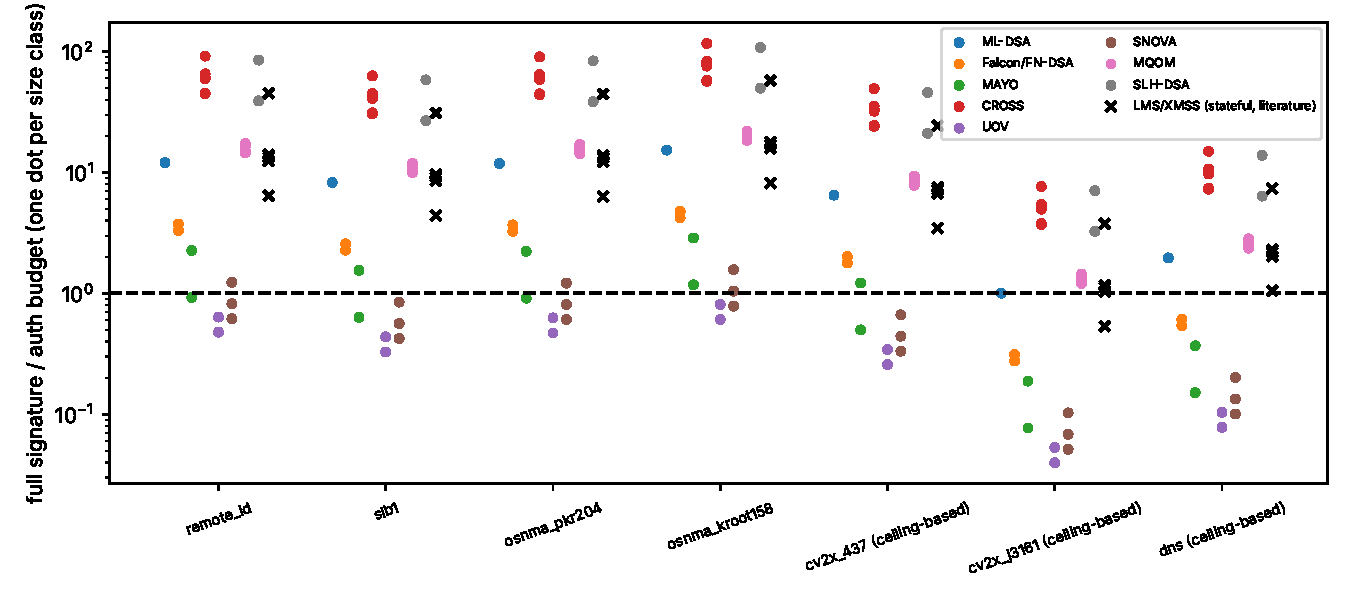
\includegraphics[width=\textwidth]{fig_q1_share.pdf}
\caption{Authentication bytes divided by budget, one dot per PQ parameter
set, per profile and mode (log scale). Points below the dashed line fit.
Provisional smoke-test data.}
\label{fig:q1}
\end{figure*}

\begin{table}[t]
\centering
\caption{Fitting parameter sets / sets in family. CROSS, ML-DSA, MQOM and
SLH-DSA fit no profile in any mode; sig\_cert fits nowhere and is omitted.}
\label{tab:q1}
\setlength{\tabcolsep}{3pt}
\begin{tabular}{@{}llccccc@{}}
\toprule
Family & Mode & C-V2X & RID & OSNMA & SIB1 & DNS \\
\midrule
\TabQOneRows
\bottomrule
\end{tabular}
\end{table}

Fig.~\ref{fig:q1} and Table~\ref{tab:q1} summarize the scoring. A full
signature fits in \QOneFullFit{} of \QOnePairs{} (parameter set, profile)
pairs: \FitCV{} for C-V2X, \FitRID{} for Remote ID, \FitOS{} for OSNMA,
\FitSIB{} for SIB1 and \FitDNS{} for DNS. Every fitting set is UOV,
SNOVA, MAYO, or (for DNS only) Falcon-512 and Falcon-padded-512. No
ML-DSA, SLH-DSA, CROSS or MQOM set fits any profile, even DNS. MAYO-2 is
the only MAYO set below the four smaller budgets.

Attaching a certificate removes every option: sig\_cert fits in
\QOneCertFit{} of \QOnePairs{} pairs, because the schemes with small
signatures have public keys of hundreds of bytes to megabytes. Broadcast
PQ authentication in these profiles therefore needs keys and
certificates distributed out of band or amortized, which is the setting
of \cite{twardokus2024when,darzi2026a}.

The PQ-anchored chain fits in \QOneChainFit{} pairs, fewer than the full
signature. Its per-message cost is small (Fig.~\ref{fig:q1}), but our
fit rule also requires the anchor signature to fit the budget, so the
chain inherits the size constraint of its anchor in the smallest
profiles (Remote ID, OSNMA). The chain's benefit is per-message cost and
loss behaviour (Q2), not a wider set of usable schemes. Hybrid mode
loses further sets in C-V2X, Remote ID and OSNMA where the classical signature
pushes the total over budget. Fragmentation does not change fit counts,
since it adds bytes; it only spreads them over frames.

\subsection{Q2: chain vs.\ fragmented under loss}

\begin{figure*}[t]
\centering
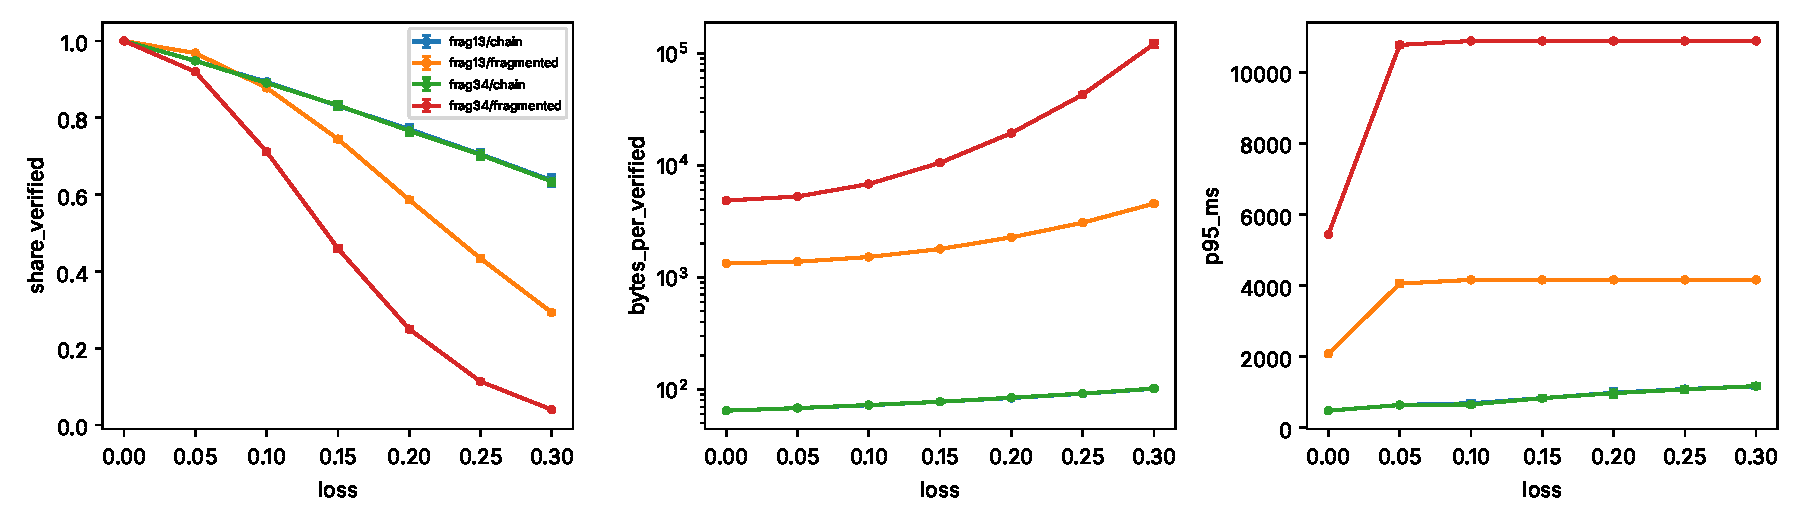
\includegraphics[width=\textwidth]{fig_q2_loss.pdf}
\caption{Loss model (Q2): share of messages verified, bytes per verified
message (log), and p95 time to authenticate (ms) versus i.i.d.\ loss.
Mean $\pm$ std over \QTwoSeeds{} seeds. Chain parameters are assumed;
see Sec.~\ref{sec:method}. Provisional.}
\label{fig:q2}
\end{figure*}

Without loss, the chain costs \BpvChainZero\,B per verified message in
the cited scenarios (\BpvChainZeroOQS\,B with the measured MAYO-1
anchor), against \BpvFragZeroFn\,B and \BpvFragZeroMl\,B for fragmented
FN-DSA and ML-DSA; p95 time is \PNFChainZero\,ms against \PNFFragZeroFn\,ms
and \PNFFragZeroMl\,ms (Fig.~\ref{fig:q2}).

At 10\% loss the chain verifies \ShChainTenFn{} of messages at
\BpvChainTenFn\,B each, versus \ShFragTenFn{} at \BpvFragTenFn\,B for
13-fragment FN-DSA, and \ShChainTenMl{} at \BpvChainTenMl\,B versus
\ShFragTenMl{} at \BpvFragTenMl\,B for 34-fragment ML-DSA. At 30\% loss
the gap widens: \ShChainThirtyFn{} versus \ShFragThirtyFn{} (FN-DSA) and
\ShChainThirtyMl{} versus \ShFragThirtyMl{} (ML-DSA), at
\BpvChainThirtyMl\,B versus \BpvFragThirtyMl\,B per verified ML-DSA
message.

The result is not uniform. Counting cells with loss $>0$ where the chain is
better by more than two standard deviations, it wins on bytes per
verified message in \QTwoBytesWins/\QTwoCells{} cells and on p95 time in
\QTwoPNFWins/\QTwoCells{}, but on verified share in only
\QTwoShareWins/\QTwoCells{}. At 5\% loss with \QTwoKfn{} fragments, fragmented
signatures verify a larger share than the chain (\ShFragFiveFn{} versus
\ShChainFiveFn{}). We have not isolated the cause; a plausible one is
that a chain message also fails when its disclosed key or anchor is lost. In a one-at-a-time sweep of $r$, $d$, $E$ and $a$
at 5, 10 and 30\% loss, the chain is better on share in
\SweepShareWins/\SweepCells{} cells and on bytes and p95 in
\SweepBytesWins/\SweepCells{} each. The p95 comparison also flatters
fragmentation: p95 is taken over verified messages only and is capped by
the deadline (\QTwoDeadFn\,ms and \QTwoDeadMl\,ms), so a low verified
share hides long waits.

We therefore do not claim that the chain dominates. Under these smoke
assumptions it is clearly cheaper in bytes and faster, and it verifies
more messages except at low loss with few fragments. We could not
reproduce the 10\%-loss point of \cite{darzi2026a} (about 41\,B versus
1971\,B retransmission overhead), because that work uses a retransmission
accounting our carousel model does not implement (\DarziTenRepro).

\subsection{Q3: is size or the timing tail binding?}

\begin{figure}[t]
\centering
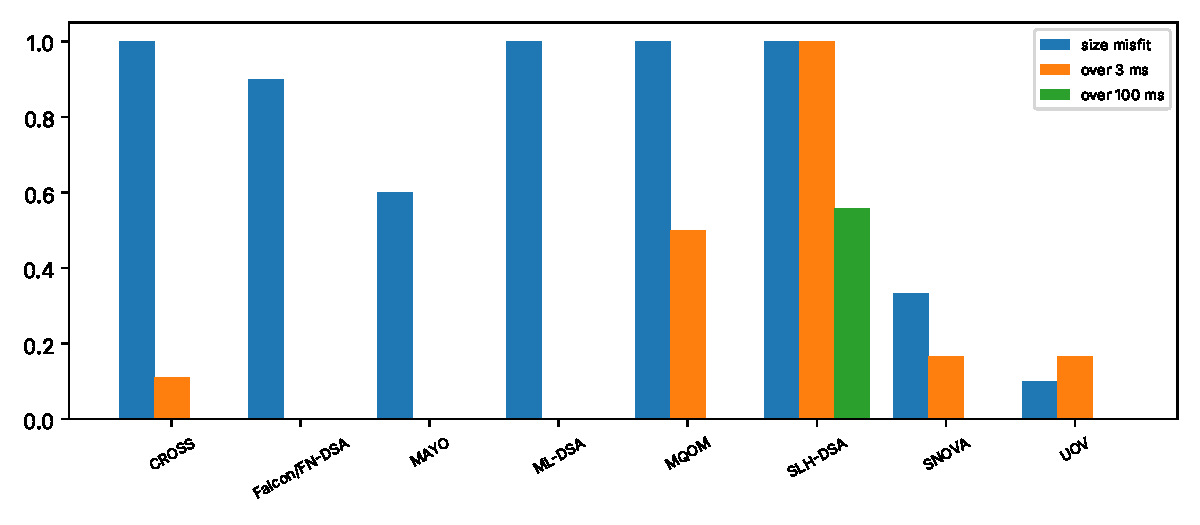
\includegraphics[width=\columnwidth]{fig_q3_size_vs_tail.pdf}
\caption{Per family: fraction of (set, profile) pairs where the full
signature does not fit, and fraction of sets whose sign or verify tail
exceeds \DeadShort\,ms or \DeadLong\,ms. x86 cloud VM only. Provisional.}
\label{fig:q3}
\end{figure}

\begin{table}[t]
\centering
\caption{Size misfit versus deadline miss per family (x86). $^\dagger$Median
of \IterSlow{} samples; tail not estimable.}
\label{tab:q3}
\setlength{\tabcolsep}{3pt}
\begin{tabular}{@{}lrlrrr@{}}
\toprule
Family & Sets & Basis & Misfit & $>$\DeadShort\,ms & $>$\DeadLong\,ms \\
\midrule
\TabQThreeRows
\bottomrule
\end{tabular}
\end{table}

Size misfit exceeds the deadline-miss fraction at both deadlines in
\QThreeSizeFams{} of \QThreeFams{} families (Table~\ref{tab:q3},
Fig.~\ref{fig:q3}); no family is timing-bound at both deadlines. Two
families qualify this. SLH-DSA is a tie at \DeadShort\,ms: every set misses both
the budgets and the \DeadShort\,ms deadline. For UOV the \DeadShort\,ms miss fraction
(\UOVOverShort) is larger than the size misfit (\UOVMisfit); the misses
come from the pkc-skc variants with sign tails of several milliseconds.
For a \DeadShort\,ms application such as sampled-value protection, UOV parameter
set choice is thus timing-constrained, not size-constrained.

This answer holds on x86 only. On microcontrollers, timings may be much larger \todo{cite or measure:
Cortex-M sign/verify for UOV, SNOVA, MAYO; chhetri2026benchmarking covers
ML-DSA only}, which could make timing binding; we did not measure this.

% ======================================================================
\section{Limitations}
\label{sec:limits}

\begin{itemize}
\item \textbf{Provisional data.} All numbers are smoke-test runs on a
  shared cloud VM (CPU: \RunCPU) with \IterFast{} iterations
  (\IterSlow{} for CROSS, MQOM, SLH-DSA). Publication runs with
  \IterFastPlanned{} and \IterSlowPlanned{} iterations on target machines
  are pending.
\item \textbf{Slow-family tails.} For CROSS, MQOM and SLH-DSA, p95/p99 are
  near-maxima of \IterSlow{} samples and Q3 uses medians for them.
\item \textbf{Q2 is inconclusive.} Results depend on assumed $r$, $d$,
  $E$, $a$ and key size, on i.i.d.\ loss (no burst loss), and on fragment
  counts $k$ taken from \cite{darzi2026a} rather than recomputed from each
  profile's payload.
\item \textbf{Q3 is x86 only.} MCU timing is not measured; the conclusion
  does not cover constrained devices.
\item \textbf{Incomplete profiles.} Fragment headers for C-V2X, SIB1 and
  DNS are unknown (\HdrCV, \HdrSIB, \HdrDNS) and set to 0. The OSNMA
  budget is derived; the 67/71 DSM-block figures of
  \cite{junquera2023assessment} are not reproduced (\JunqueraBlocksRepro),
  and our block arithmetic does not match them without the full text.
  Three of the four Q1 chain parameters (key, commitment, timestamp
  sizes) are assumed, not cited.
\item \textbf{Baselines not reproduced.} The 34/13 SIB1 fragments and
  324\,B overhead of \cite{darzi2026a} (\DarziFragRepro) and its 10\%-loss
  point (\DarziTenRepro); the ZK compression of \cite{yoshizawa2026a}
  (\YoshizawaRepro); the DNS transfer sizes of \cite{goertzen2022post}
  (\GoertzenRepro); and the size tables of \cite{chen2025hybrid}.
\item \textbf{Scope.} Stateful hash-based signatures (LMS/XMSS) are not
  benchmarked. ETSI ITS, ADS-B, AIS and LoRaWAN profiles are not
  included. Security of the modes (e.g.\ hybrid downgrade, time
  synchronization attacks on the chain) is not analysed.
\item \textbf{Related work.} Several related papers, including the
  closest competitor \cite{hyoung2026post}, were read as abstracts only.
\end{itemize}

% ======================================================================
\section{Conclusion}

Scoring one set of authentication modes against five handshake-free
broadcast budgets shows, in provisional x86 data, that only UOV, SNOVA,
MAYO and two Falcon parameter sets fit any profile with a full
signature, that no set fits with a same-scheme certificate, and that
size rather than x86 timing is usually the binding constraint. A
PQ-anchored key chain is far cheaper per verified message than
fragmented signatures under loss, but it does not verify more messages
at low loss and the comparison rests on assumed parameters. Next steps
are publication runs on target hardware including microcontrollers,
recomputed fragment counts, burst loss, and reproduction of the
\cite{darzi2026a} and \cite{junquera2023assessment} baselines.

\section*{Artifact}
Scripts that regenerate every number in this paper from raw CSVs:
\todo{artifact URL}.

\bibliographystyle{IEEEtran}
\bibliography{../../../research/lit/refs}

\end{document}
